
\section{Introduction}
The algorithmic trading of stock shares can be triggered by high complex event patterns that are specified 
based on patterns in the event stream of the stock market. Such algorithmic trading mostly is specified 
based on the history of the event stream, for example, by utilizing moving averages of stock prices and the trading volumes. 
The real-time extraction of such complex patterns to trigger buy or sell trading actions is the task 
of high-performance event stream processing systems. 

% Describe briefly what the challenge is 
This year's DEBS Grand Challenge \cite{debs2022challenge} describes a system implementation based on two specific queries on the 
stock market event streams. The first query is defined to compute the Exponential Moving Average (EMA) with two 
different smoothing factors of 38 and 100. 
An exponential Moving Average is one of the moving averages and is defined as follows:

\begin{align*}
    EMA_t = \begin{cases} 
        Y_0 &  t = 0 \\ 
        \alpha Y_t + (1-\alpha) EMA_{t-1}& t>0 \\ 
        \end{cases}
\end{align*}

The coefficient $\alpha$ represents the degree of weighting decrease, a constant smoothing factor between 0 and 1.
For this challenge $\alpha = \frac{2}{1+j}$ where $j$ is a smoothing factor with $j \in \{38, 100 \}$.
We use $EMA_{38}$ to refer to the exponential moving average with a smoothing factor of 38 
and $EMA_{100}$ for a smoothing factor of 100. 


\begin{figure}[!ht]
    \begin{center}
        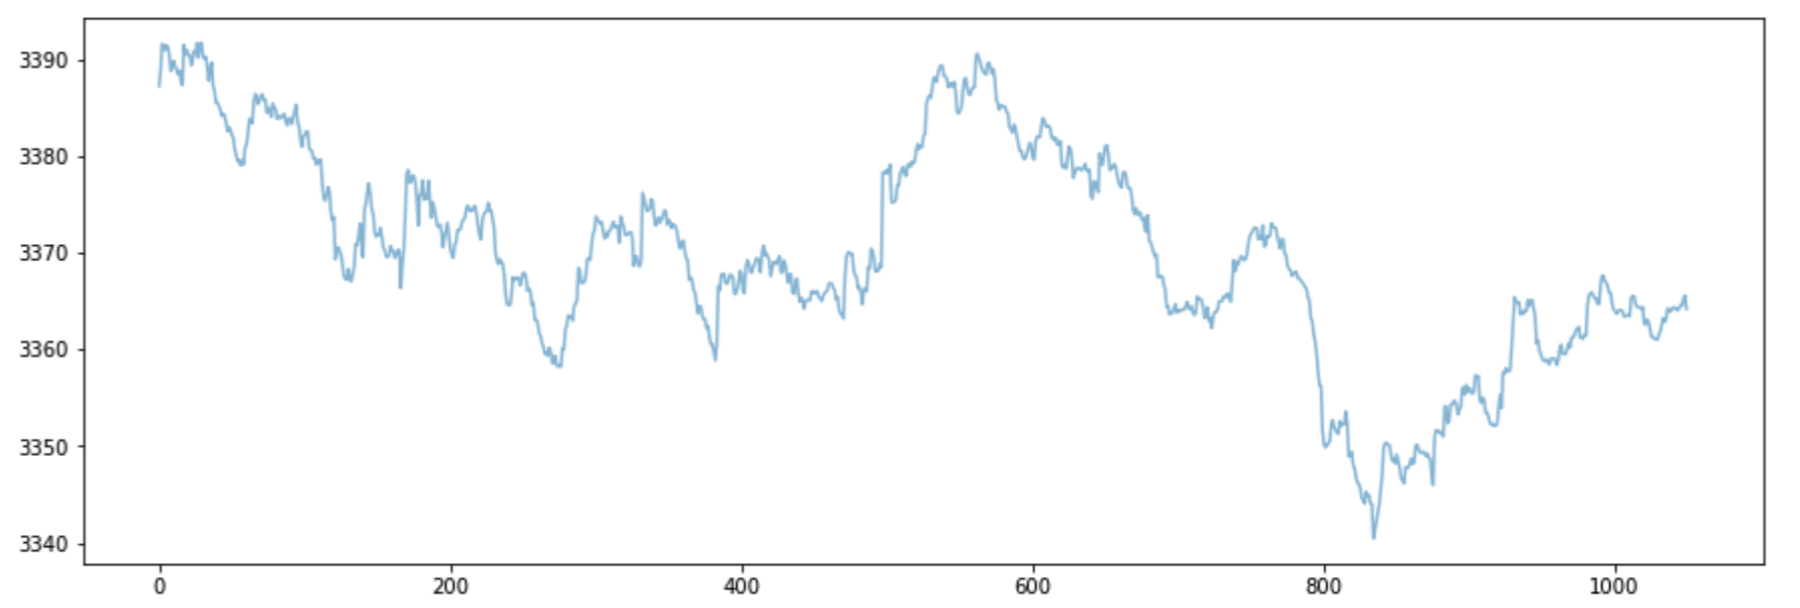
\includegraphics[width=0.42\textwidth]{./images/stock_example.png}
        \caption{An Example of Stock Price Fluctuations Over Time}
        \label{fig:stock}
    \end{center}
\end{figure}



\begin{figure*}[!ht]
    \begin{center}
        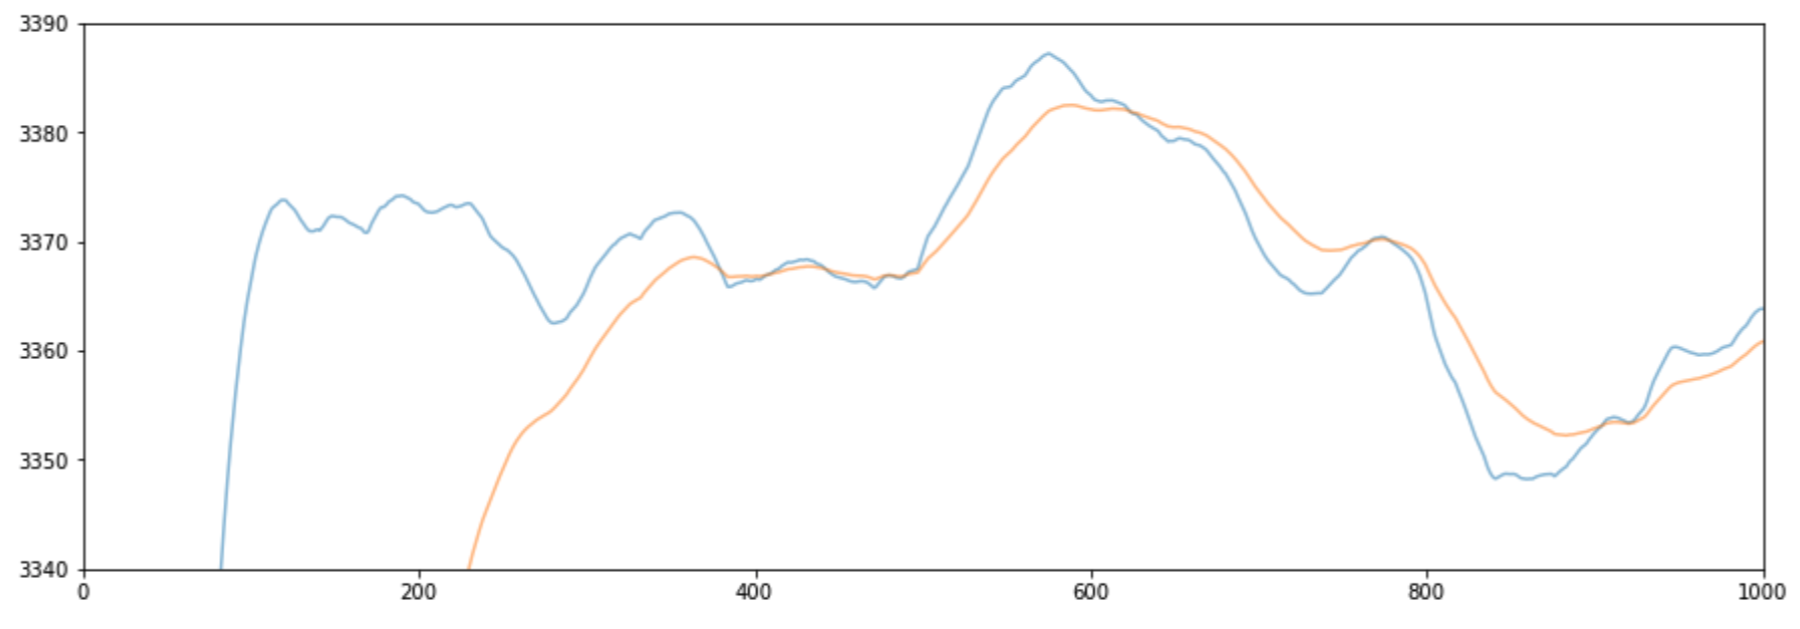
\includegraphics[width=0.70\textwidth]{./images/query2_example.png}
        \caption{Example of Query 2 - Buy and Sell advice based on Breakout Patterns of EMA 38 and 100 }
        \label{fig:EMAs}
    \end{center}
\end{figure*}


% Describe the query 1 and 2 
Figure \ref{fig:stock} illustrates an example of stock market price changes over time. The graph shows 1000 events with 
different prices. Figure \ref{fig:EMA200} depicts the values of the exponential moving average with 
smoothing factors of 38 and 100. We can observe in Figure \ref{fig:EMA200} how the value grows exponentially 
and how the two $EMA_{38}$ and $EMA_{100}$ are different from each other. 

Query 2 of the DEBS2022 challenge \cite{debs2022challenge} is specified based on the results of query 1. Each time 
that $EMA_{38}$ breaks out of the value of $EMA_{100}$ a stock buy advice notification should be generated and if
$EMA_{100}$ goes under the $EMA_{38}$ a stock sell advice. For a further detailed description of the DEBS 2022 
Grand Challenge, we would refer the readers to \cite{debs2022challenge}. 

Figure \ref{fig:EMAs} visualize the same graph as we have in Figure \label{fig:EMAs} by 
zooming into the graph (range 0 to 200 events on x-axis) to see the values and their differentiations. One important observation in 
Figure \ref{fig:EMA200,fig:EMAs} is that $EMA_{38}$ and $EMA_{100}$ have a large difference in the first 
200 events.  The reason for this difference is that the exponential moving average is specified based 
on the history of events to increase the value exponentially and requires a warm-up phase. Based on this observation,
one can improve the performance of the query 2 by skipping the first 200 events for query 2 because 
$EMA_{38}$ and $EMA_{100}$ have still a large difference. 

The main system development challenge task is to design a system that can process the stream of events with high throughput and low latency. 
Many open source and commercial stream processing systems are developed that one can use to develop this challenge. 
Esper event stream processing system \cite{Bernhardt2007} is a system that can detect complex events based on pre-defined temporal logic patterns. 
In this task we do not have a complex pattern to extract and computation are basic computation of EMA 38 and 100, and a subsequent check if the values for 
query 2 to submit a sell or buy advice. Other systems like Apache Storm \cite{8288619}, Apache Spark Streaming \cite{zaharia2010spark} or 
Apache Flink streaming \cite{alexandrov2014stratosphere} are developed to achieve high-scalability in processing the data stream. 
Also, different benchmarks are developed  \cite{8701904} which compare these systems with each other regarding specific data 
stream processing tasks. 

After considering all of the existing systems and their overhead trade-offs, we decided to implement the DEBS grand challenge from scratch and 
without using any of the existing systems because most of them have a different target with a large start-up delay which might impact 
our stream processing performance. The first implementation is a prototype of the system in python because we would like to make sure 
that we understand the logic of these two queries and can run tests to check if the data streams are processed correctly, and the correct 
trading advices are submitted to the DEBS2022 evaluation system. 


% High-Performance computing problems 
% Scalability issues 

\begin{figure}[!ht]
    \begin{center}
        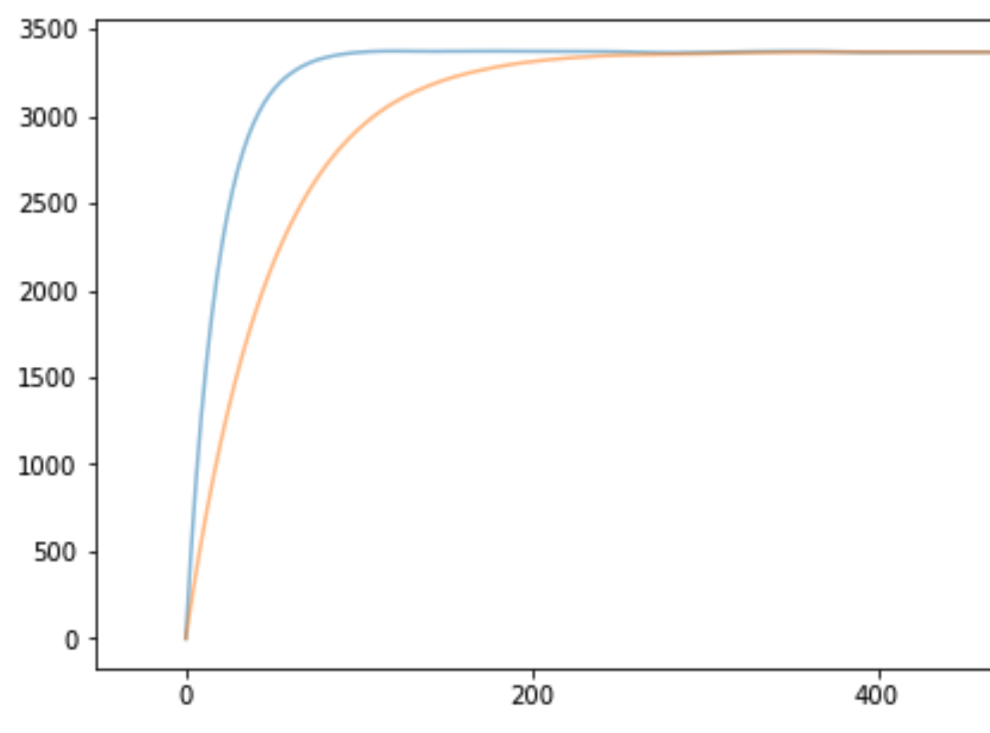
\includegraphics[width=0.4\textwidth]{./images/query2_example_200.png}
        \caption{Exponential Moving Average of 38 and 100 for the first 400 events.}
        \label{fig:EMA200}
    \end{center}
\end{figure}


The next subsequent sections describe details of our implementation. Section \ref{sec:concepts} describes our ideas for 
stream processing using multiple processing threads on a single machine with multiple CPU cores. Further we describe how the same 
architecture can be extended to process the data stream on a cluster of machines.  Section \ref{sec:implementation} provides 
a brief description of important implementation details and Section \ref{sec:experiments} provides a brief overview of different 
experiments.


